\section{Performance + Portability}
\label{sec:pp}

Until now, I looked at performance and portability as separate instances. 
If one knows that the code will only ever be executed on one specific hardware platform, achieving the best performance possible down to the assembly level is essential and may be desirable. 
On the other hand, writing code that can be executed everywhere while sacrificing a bit of performance may be enough for some. 
However, in many cases, especially in \gls{hpc}, achieving a combination of both performance and portability is also essential: writing code that can be executed on various hardware platforms without the need to re-implement everything from scratch again if the hardware changes and that also achieves reasonable performance on all hardware platforms is important. 
Reasonable means achieving a high enough fraction of the achievable peak performance. 
It should be clear that it is extremely difficult or even impossible to achieve the same performance with code that can run on all \glspl{gpu} and \glspl{cpu} there are compared to highly optimized vendor-specific solutions that may even be implemented by the vendors themselves with special closed-source knowledge of the underlying hardware. 

Assessing performance portability is an ongoing research topic. 
In the following subsections, I will discuss the history of performance portability, starting with its informal beginnings, through the first performance portability metric, up to the current state of the art. 
Additionally, I will introduce the new heterogeneity score, which complements the performance portability by specifying how representative our used hardware platforms are with respect to the platforms we ultimately want to support. 
This section is closed with an example of the different performance portability metrics based on three artificial example applications and a possible way to visualize the performance portability proposed by~\citet{sewall_interpreting_2020}.

\subsection{The Pre Performance Portability Metrics Era (-- 2016)}
\label{sec:pre_pp_era}


Since more than three decades now is the computer science community concerned with performance portability~\cite{bailey_nas_1991, irigoin_performance_1994, strazdins_high_1996, foster_performance_1996, reed_portability_1996, ngo_portable_1997, jiang_application_1997, cermele_performance_1998, zaafrani_performance_1999, michalakes_performance-portability_2001, goos_achieving_2001, ko_frame_2002, worley_performance_2005, jones_practical_2005, komatsu_evaluating_2010, gabriel_towards_2010} also indicated by the first Workshop on Portability and Performance for Parallel Processing in 1993~\cite{hey_portability_1994}. 
In this era, whenever a new computer architecture or paradigm emerged, like new \gls{cpu} architectures, the introduction of many-core processors, or distributed memory systems, the question arised whether it is possible to target these new systems in a portable but also performant way and if so how that could be achieved. 
However, these concerns were never tackled formally until \citet{zhu_performance_2007} introduced the first quantitative formula regarding performance portability in their paper in \citeyear{zhu_performance_2007}. 
However, this first metric was only usable in a very narrow setting. 
\citeauthor{zhu_performance_2007} defined their performance portability as:
\begin{quotebox}{\citet{zhu_performance_2007}}
    If one parallel implementation of one application already achieves good performance on one platform, can this implementation also achieve the same or similar performance on other platforms?
\end{quotebox}
They used this informal definition to derive the first but also somewhat limited performance portability metric:

\begin{definition}[Performance Portability $P^\mathcal{P}_n(b \rightarrow t$)~\cite{zhu_performance_2007}]
Given a parallel program $\mathcal{P}$ developed on the \textbf{base system}, let $S^B_n$ denote the absolute speedup achieved by $\mathcal{P}$ on $n$ computing nodes of the \textbf{base system}, and $S^T_n$ denote the absolute speedup achieved by $\mathcal{P}$ on $n$ computing nodes of the \textbf{target system}, then the \textbf{performance portability} on $n$ computing nodes for porting the program $\mathcal{P}$ from the \textbf{base system} to the \textbf{target system} is:

$$P^\mathcal{P}_n(b \rightarrow t) = \frac{S^T_n}{S^B_n} \times \SI{100}{\percent}$$
\end{definition}

While this was the first quantitative performance portability definition, it lacks generalizability since it is really only meant for code running on compute clusters with multiple nodes. 
\citeauthor{zhu_performance_2007} also mention this limitation in their paper as they define performance portability in the context of speedup since they argue that the performance is portable with an increasing number of compute nodes. 
While this definition of performance portability may have been sufficient at the time, it lacks behind in the current time where programmers have to not only factor in different \gls{cpu} architectures, \gls{cpu} core counts, or number of compute nodes, but also completely different hardware architectures like \glspl{gpgpu}, \glspl{fpga}, or \glspl{tpu} from different vendors.
Since the computational power of these different hardware architectures varies significantly, and some architectures are vastly superior to others depending on the problem at hand, concerns about performance portability further increased. 

To discuss performance portability in different contexts with different people, possibly from different domains, it is necessary to have a purely subjective, quantifiable metric on which everyone can agree. 
However, even after the success story of modern \glspl{gpgpu}, performance portability was still only tackled with informal and subjective definitions in the first years. 
Note that the following definitions are not an exhaustive list but only serve as examples.

In \citeyear{edwards_kokkos_2013} in their original Kokkos paper \citet{edwards_kokkos_2013} defined performance portability as:
\begin{quotebox}{\citet{edwards_kokkos_2013}}
    Our performance portability objective is to maximize the amount of user code that can be compiled for diverse devices and obtain the same (or nearly the same) performance as a variant of the code that is written specifically for that device.
\end{quotebox}
Although this definition is already quite good, the problem is that \enquote{\textit{nearly the same}} can and will be interpreted differently by different people. 
Therefore, this definition is not feasible for object performance portability measurements.

A year later, in 2014 \citet{kunkel_performance_2014} defined performance portability as:
\begin{quotebox}{\citet{kunkel_performance_2014}}
    A code is performance portable if it can achieve a similar fraction of peak hardware performance on a range of different target architectures.
\end{quotebox}
As with the quote from \citeauthor{edwards_kokkos_2013}, the problem is the objectivity of the definition, namely how big the \enquote{\textit{similar fraction of}} should be. 
Although \citeauthor{kunkel_performance_2014} stated that for them it is $\SI{20}{\percent}$ of the best achievable performance with respect to a hand-optimized native implementation, another person could argue that it should be $\SI{15}{\percent}$ or $\SI{25}{\percent}$ making this definition also highly subjective. 

In \citeyear{larkin_performance_2016}, \citet{larkin_performance_2016} defined performance portability as:
\begin{quotebox}{\citet{larkin_performance_2016}}
    The same source code will run productively on a variety of different architectures.
\end{quotebox}
Again, \enquote{\textit{productively}} is highly subjective in a performance and portable or productive way since this definition can include that maintaining custom code paths for better performance may be okay if it is not too much work, defeating the portability aspect of performance portability. 


Later that year, due to the increasing necessity of developing a performance portability definition, the \gls{doe} in the United States conducted a meeting~\cite{neely_doe_2016} specifically regarding performance portability. 
There, a few attendees were asked to define performance portability in their own words:
\begin{quotebox}{Rob Neely~\cite{neely_doe_2016}}
    For purposes of this meeting, it is the ability to run an application with acceptable performance across KNL and GPU-based systems with a single version of source code.
\end{quotebox}
\begin{quotebox}{Simon Pennycook~\cite{neely_doe_2016}}
    An application is performance portable if it achieves a consistent level of performance (e.g., defined by execution time or other figure of merit, not percentage of peak flops across platforms relative to the best known implementation on each platform.
\end{quotebox}
\begin{quotebox}{Adrian Pope, Vitali Morozov~\cite{neely_doe_2016}}
    Hard portability = no code changes and no tuning. Software portability = simple code mods with no algorithmic changes. Non-portable = algorithmic changes.
\end{quotebox}
\begin{quotebox}{David Richards~\cite{neely_doe_2016}}
    A code is performance portable when the application team says its performance portable!
\end{quotebox}

At the end of the \gls{doe} meeting, the attendees also created a working definition trying to incorporate the above definitions into one: 
\begin{quotebox}{\gls{doe} Working Definition~\cite{doe_meeting_attendees_definition_2016}}
    An application is performance portable if it achieves a consistent ratio of the actual time to solution to either the best-known or the theoretical best time to solution on each platform with minimal platform specific code required.
\end{quotebox} % https://performanceportability.org/perfport/definition/
As with all previous definitions, these quotes contain some objective part in one way or another and are not suited for an objective performance portability metric. 
This led \citeauthor{pennycook_metric_2016} later in the same year to create the first general-purpose performance portability metric, making it for the first time ever possible to discuss the performance and portability of different applications on different hardware platforms in an objective manner. 

\subsection{The First Performance Portability Metric \pp (2016 -- 2017)}
\label{sec:first_pp_metric}

\todo{Übergänge}

The first version of the performance portability metric developed by \citet{pennycook_metric_2016} was developed as a preprint in \citeyear{pennycook_metric_2016}. 
A revised version of the paper~\cite{pennycook_implications_2019} was submitted to Elsevier Science in 2017 and finally published in the Future Generation Computer Systems Periodical in~\citeyear{pennycook_implications_2019}. 

\citeauthor{pennycook_implications_2019} define the following terms also used in their later definitions and formulas. 
A \textit{platform} $\mathbf{i}$ is a particular execution environment, mostly interpreted as a specific hardware platform; the set of all possible platforms is denoted as $\mathbf{H}$. 
An \textit{application} $\mathbf{a}$ is any software, library, or source code that can accept a \textit{problem} $\mathbf{p}$ as input and produce an output that can be validated against a known ground truth. 
Based on these terms, \citeauthor{pennycook_implications_2019} define the \textit{performance}  
\begin{quotebox}{\citet{pennycook_implications_2019}}
    Any measurable property of an application’s correct execution of a problem on a platform.
\end{quotebox}
and the \textit{portability} 
\begin{quotebox}{\citet{pennycook_implications_2019}}
    The ability of an application to execute a problem correctly on a given set of platforms.
\end{quotebox}
of an application solving a specific problem on a given platform. 

The foundation of the performance portability metric, as described by \citeauthor{pennycook_implications_2019}, is the observation of three key points, also emphasized during the previously mentioned \gls{doe} meeting, that must be fulfilled for any performance portability metric to be feasible:
\begin{enumerate}
    \item Reflect the individual meanings of the terms \textit{performance} and \textit{portability};
    \item Be objective;
    \item Be measurable (and comparisons of the measured value should be meaningful).
\end{enumerate}
Especially points 2. and 3. disqualify all definitions mentioned in the previous \autoref{sec:pre_pp_era}.
Based on these criteria, \citeauthor{pennycook_implications_2019} devised their own informal definition of performance portability: 
\begin{quotebox}{\citet{pennycook_implications_2019}}
    A measurement of an application’s performance efficiency for a given problem that can be executed correctly on all platforms in a given set.
\end{quotebox}
In contrast to the previous informal definitions, this one is objective since it specifies that the \textit{performance efficiency} measurement, i.e., the ratio of some observed performance with respect to some known, achievable level of performance, should be used to determine whether an application has \enquote{good} performance or not. 

\citeauthor{pennycook_implications_2019} also directly provide two definitions of performance efficiency that will become important later. 
Both definitions define the performance efficiency of an application $\mathbf{a}$ solving problem $\mathbf{p}$ on the hardware platform $\mathbf{i \in H}$. 
Both definitions' values lie in the range $\interval{0}{1}$, where $1$ denotes the observed performance is equal to the best possible performance, and lower values mean that the performance further degrades. 

\begin{definition}[Architectural Efficiency]\label{def:arch_eff}
    The achieved performance as a fraction of the \enquote{peak} theoretical hardware performance, e.g., the achieved \si{\flop\per\second} or memory bandwidth.
\end{definition}

The \textit{architectural efficiency} represents an application's ability to utilize the available hardware. 
Note that an architectural efficiency of $1$, i.e., achieving, for example, $\SI{100}{\percent}$ of the available peak memory bandwidth, does not mean that an application is perfectly optimized since it is very well possible that the application performs many unnecessary loads artificially increasing the utilized memory bandwidth. 

\begin{definition}[Application Efficiency~\cite{satish_can_2012}]\label{def:app_eff}
    The achieved performance as a fraction of the \enquote{best} observed performance. 
\end{definition}

The \textit{application efficiency} represents an application's ability to use the best-known implementation or algorithm for each platform. 
Again, an application efficiency of $1$ does not mean that an application achieves the best performance possible since the best \textit{known} performance may not be the best performance that \textit{may be possible}.
Also, both performance efficiencies are complementary, and using both efficiencies achieves the best explainability of the results. 
The interpretation of the results is straightforward if both performance efficiencies are small or big.
On the other hand, if an application's architectural efficiency is high while its application efficiency is low, the results indicate that the hardware resources are only used poorly. 
In contrast, a high application efficiency and a low architectural efficiency may suggest that all implementations, including the best-known implementation, can be further improved. 

Finally, \citeauthor{pennycook_implications_2019} devised five criteria that directly influence the design of their performance portability metric definition.
\begin{definition}[Performance Portability Criteria~\cite{pennycook_implications_2019}]\label{def:pp_criteria}
    \begin{enumerate}
        \item Be measured specific to a set of platforms of interest $\mathbf{H}$.
        \item Be independent of the absolute performance across $\mathbf{H}$.
        \item Be zero if a platform in $\mathbf{H}$ is unsupported, and approach zero as the performance of platforms in $\mathbf{H}$ approaches zero. 
        \item Increase if performance increases on any platform in $\mathbf{H}$.
        \item Be directly proportional to the sum of scores across $\mathbf{H}$.
    \end{enumerate}
\end{definition}
These criteria directly led to the first formal, general-purpose performance portability metric:

\begin{definition}[Performance Portability \pp~\cite{pennycook_implications_2019}]\label{def:pp}
    Given a problem $\mathbf{p}$ which is solved by an application $\mathbf{a}$ and a set of platforms $\mathbf{H}$, the performance portability metric \pp is defined as:

    \[ \pp(a, p, H) = 
        \begin{cases}
            \frac{\abs{H}}{\sum\limits_{i \in H} \frac{1}{e_i(a, p)}} & \text{if }i\text{ is supported } \forall i \in H \\
            0                                                         & \text{otherwise}
        \end{cases} 
    \]

    where $\mathbf{e_i}$ is the performance efficiency of $\mathbf{a}$ solving $\mathbf{p}$ on platform $\mathbf{i \in H}$.
\end{definition}

Therefore, the performance portability metric \pp is the harmonic mean over the performance efficiency of an application solving a specific problem on all tested hardware platforms. 
The only difference to the harmonic mean is that \pp is also defined if the performance efficiencies include one or more zeros, i.e., an application did not run on one or more hardware platforms in $\mathbf{H}$. 
The \pp metric has the nice property that, per construction, it is in the interval $\interval{0}{1}$ where $0$ means the application did not run on all hardware platforms and $1$ means the best possible performance on all hardware platforms could be achieved. 
Note that \pp heavily emphasizes the \textit{portability} aspect of performance portability: If only one hardware platform is not supported, the resulting \pp value will be $0$ regardless of the performance on all other hardware platforms. 
Depending on your target audience, this property of \pp may or may not be desirable. 
This \autoref{def:pp} laid the foundation for many researchers in the following years.

\subsection{Performance Portability Metrics Revised (2017 -- 2022)}
\label{sec:pp_revised}

Many researchers adopted the \pp metric in their work in the following years~\cite{kirk_achieving_2017, hsu_performance_2018, pennycook_evaluating_2018, zhao_delivering_2018, yang_empirical_2018, yokota_beginners_2018, sedova_high-performance_2018, harrell_effective_2018, deakin_performance_2019, reguly_performance_2019, daniel_applying_2019, deakin_tracking_2020, bertoni_performance_2020, grete_k-athena_2021, deakin_analyzing_2021, ibrahim_performance_2022, dieguez_ml-based_2022, breyer_performance_2023, marowka_toward_2023, ernstsson_assessing_2023, rangel_performance-portable_2023, davis_taking_2024, crisci_minilb_2024, lorenzon_towards_2024, asahi_development_2024, guerrero_study_2025}, further underlining the necessity of such an objective performance portability metric. 
But the \pp metric was not only used by other researchers; they also tried highlighting potential problems with \pp and solutions, as well as improvements and extensions. 

For example, \citet{harrell_effective_2018} noted in \citeyear{harrell_effective_2018} that \pp tracks performance and portability but completely ignores the third P, productivity. 
It especially does not penalize heroic optimization efforts, i.e., highly optimized divergent code paths for specific architectures, to increase the \pp score, which certainly would reduce the productivity due to the necessity to maintain said code paths. 
Therefore, \citeauthor{harrell_effective_2018} extended the performance portability further to an \textit{effective performance portability} by introducing a \textit{code divergence} measurement. 
However, since productivity is subjective, depends on a programmer's experience with the frameworks used, and should already be tracked during development either manually or using automatic tools~\cite{harrell_effective_2018}, I will only focus on the performance portability aspect in this work and ignore productivity. 

The work of \citet{daniel_applying_2019} in \citeyear{daniel_applying_2019} combines the \pp metric of \citet{pennycook_evaluating_2018} with the code divergence of \citet{harrell_effective_2018}. 
Their main interest was the observation that the performance and performance portability also depend on the input size of the problem $\mathbf{p}$, which \pp currently ignores. 
Instead of using the code distance as \citeauthor{harrell_effective_2018} did, they define a \textit{performance distance} that can either be based on the architectural or application efficiencies. 
\citeauthor{daniel_applying_2019} final \textit{performance portability divergence} $P_\mathcal{D}$ is then defined as the root mean squared error of all performance distances between the set of input sizes of interest with respect to the set of target platforms. 
It should be noted that the optimal value of $P_\mathcal{D}$ is $0$, which is easier to reach than $1$ with \pp~\cite{daniel_applying_2019}. 

In \citeyear{sedova_high-performance_2018}, \citet{sedova_high-performance_2018} also created a new performance portability metric measuring the performance portability on a programmatic level since they also argue that \pp does not penalize non-portable but highly optimized code paths. 
If the value of their $PP_{MD_c}$ metric (here, $MD$ stands for molecular dynamics since \citeauthor{sedova_high-performance_2018} evaluated their metric on molecular dynamic codes) is close to $0$, it means that a large part of the code must be replaced with a portable version with the same performance level to achieve real performance portability. 
However, since $PP_{MD_c}$ currently does not support results from multiple machines~\cite{sedova_high-performance_2018}, it is also excluded from this work. 

\citet{yang_empirical_2018} in \citeyear{yang_empirical_2018} also tried to improve \pp but not by changing or augmenting \pp itself but by proposing a new performance efficiency measurement in addition to the already existing architectural (\autoref{def:arch_eff}) and application (\autoref{def:app_eff}) efficiency. 
They argue that the architectural efficiency may skew the results because it uses vendor-provided theoretical and possibly over-optimistic or unreachable peak performance values. 
On the other hand, the Roofline model accounts for different architecture-specific performance bounds that may limit the observed sustained performance. 
\citeauthor{yang_empirical_2018} define the Roofline performance efficiency as: 
\begin{definition}[Roofline Performance Efficiency~\cite{yang_empirical_2018}]\label{def:roof_eff}
Given the observed code performance in floating point operations per second $\left(\si{\flop\per\second}\right)$ $P_i(a, p)$, the peak \si{\flop\per\second} $F_i$ of architecture $\mathbf{i}$, the peak bandwidth $B_i$ of architecture $\mathbf{i}$, and the arithmetic intensity $I_i(a, p)$ of application $\mathbf{a}$ on architecture $\mathbf{i}$, the Roofline performance efficiency is defined as:

$$e_i(a, p) = \frac{P_i(a, p)}{\min(F_i, B_i \times I_i(a, p))}$$
\end{definition}
However, the Roofline model and, therefore, the Roofline efficiency, suffers two major problems~\cite{bertoni_performance_2020, marowka_reformulation_2022}. 
First, establishing a correct theoretical Roofline model is highly non-trivial and an active research field~\cite{williams_roofline_2009, ilic_cache-aware_2014, yokota_novel_2018, taufer_applying_2016, hsu_performance_2018, grete_k-athena_2021, naraparaju_shifting_2024, antepara_performance_2024}. 
Second, empirically created Roofline models, e.g., using the STREAM benchmark~\cite{mccalpin_memory_1995} to determine the sustained memory bandwidth, may give different results on different machines even though the same hardware is used. 
This makes it difficult to reproduce or compare results from different publications. 

Regarding different performance efficiency measurements, \citet{siklosi_heterogeneous_2018} also argue that it becomes noticeably more difficult to get meaningful results for a heterogeneous application, i.e., an application that, e.g.,  does not only use \glspl{cpu} to offload some computation to an \gls{gpu} but that uses \glspl{cpu} and \glspl{gpu} simultaneously. 

In \citeyear{yokota_beginners_2018}, \citet{yokota_beginners_2018} analyzed the \pp metric using five case studies and highlighted some findings and problems, namely the tension between performance improvements and performance portability improvements. 
They identified three ways to improve the performance portability value. 
First, we can increase the number of platforms in the platform set $\mathbf{H}$. 
Adding new platforms for already supported types with a good efficiency will improve the value of \pp. 
However, for the discussion of performance portability in general, it may be more interesting to add new platforms of a completely different type like \glspl{gpu} from a different vendor. 
This platform heterogeneity is currently not included in the \pp metric but would be interesting when comparing the \pp scores of different platform sets. 
Second, we can reduce the number of platforms by removing platform types that are not well supported, for example, \glspl{cpu} for an application mainly developed for \glspl{gpu}. 
While this will increase the \pp score, it would also decrease the platform heterogeneity. 
Whether this is desirable heavily depends on the application and use case. 
Third, increasing the performance efficiency of the application on one or more platforms. 
Improving the performance efficiency on a platform can have multiple effects: improving efficiency on all platforms (best case) or improving efficiency only on this platform but decreasing it on all other platforms (worst case). 
\citeauthor{yokota_beginners_2018} also highlight the already mentioned problem with the architectural efficiency where a good efficiency score must not necessarily correlate with an efficient implementation.  
Therefore, they also used the application efficiency for their case studies, implementing five problems using OpenACC. 
However, this also highlighted the main problem with the application efficiency. 
They used a \gls{cuda} implementation as the best-performing baseline and implemented the same code with OpenACC. 
As a result, their OpenACC implementation was faster than the \gls{cuda} baseline, resulting in an application efficiency of $\SI{100}{\percent}$ for the OpenACC code. 
However, does this make sense? 
One can argue that \gls{cuda} as the vendor-specific low-level programming model for NVIDIA \glspl{gpu} should always be faster than the high-level OpenACC version. 
This shows the main problem with the application efficiency: selecting the correct baseline implementation is crucial to achieve a meaningful result. 
The last problem with \pp they highlight is directly caused by using the harmonic mean in \pp, which overly penalizes small performance efficiency scores, skewing the results. 
Consequently, when only reporting a small \pp score, it is impossible to determine whether all efficiencies are low or whether only a small fraction of all platforms in $\mathbf{H}$ have a low efficiency while all others are efficient. 
The same problem has also been discussed by \citet{bertoni_performance_2020}. 
They propose to additionally report the standard deviation of the achieved performance efficiencies. 

Besides \citeauthor{yokota_beginners_2018}, in \citeyear{marowka_toward_2021} \citet{marowka_toward_2021}, with an extended paper published at the beginning of 2022~\cite{marowka_reformulation_2022}, also thoroughly investigated the \pp metric and found some issues, the main one being the usage of the harmonic mean in the \autoref{def:pp} of \pp. 
He argues, and later proves, that using the harmonic mean violates the criteria $5$ from \autoref{def:pp_criteria} since \pp is not proportional to the sum of scores across $\mathbf{H}$. 
Furthermore, he states that \pp being zero if any platform is unsupported, as noted in criteria $3$, is also a direct result of using the harmonic mean. 
\citeauthor{marowka_toward_2021} concludes that the arithmetic mean is a better alternative to the harmonic mean and proposes his own performance portability metric. 

\begin{definition}[Performance Portability \mpp~\cite{marowka_toward_2021}]\label{def:mpp_provisional}
    Given a problem $\mathbf{p}$ which is solved by an application $\mathbf{a}$ and a set of supported platforms $\mathbf{H}$ from \textbf{the same architecture class}, the performance portability metric \mpp is defined as:

    \[ \mpp(a, p, H) = 
        \begin{cases}
            \frac{\sum\limits_{i \in H} e_i(a, p)}{\abs{H}} & \text{if }i\text{ is supported }\forall i \in H \\
            \textit{not applicable}                         & \text{otherwise}
        \end{cases} 
    \]

    where $\mathbf{e_i}$ is the performance efficiency of $\mathbf{a}$ solving $\mathbf{p}$ on platform $\mathbf{i \in H}$.
\end{definition}

Besides using the arithmetic mean instead of the harmonic mean, which also has the benefit of not disproportionately tracking lower values, \citeauthor{marowka_toward_2021} also changed four additional things compared to the \autoref{def:pp} of \pp. 
First, if a platform is not supported, the \mpp score is not $0$ but reported as \textit{not applicable} to explicitly distinguish it from low-performance portability values approaching $0$. 
He additionally states that setting the \pp score to $0$ only because a single platform in $\mathbf{H}$ is unsupported for the current implementation is unrealistic. 
Second, he observed that in many real-world examples, there is a noticeable gap between the performance efficiency of \glspl{cpu} and \glspl{gpu}. 
He, therefore, suggests that \mpp should only be calculated for platforms in the same architectural class, i.e., one would have to calculate different \mpp values for \glspl{cpu} and \glspl{gpu}. 
Third, for the application efficiency, if there is no known baseline implementation, the best-performing version of the current implementations is often used as a baseline and included in the \pp score, possibly skewing its results. 
For \mpp, \citeauthor{marowka_toward_2021} proposes excluding these baseline values from its calculation. 
Fourth, he states that clear outliers should be removed from the calculation but fails to specify what characterizes a clear outlier.
While some of these changes can be justified, the question of whether points two and four are desirable is especially questionable if the goal is to showcase performance portability across diverse architectures. 

In the same year, \citet{marowka_performance_2022} also proposed a variation of his \mpp metric, which is not application but programming model-centric. 
The basic idea is to report the achieved performance of a portable programming model $M$ as a fraction of the performance of a non-portable architecture-specific parallel programming model across various case studies. 
However, since the number of case studies must be relatively large to draw meaningful conclusions, this metric is more suited for meta-studies. 

Since \citeauthor{marowka_portability_2024} also criticized the architectural and application efficiencies, in \citeyear{marowka_portability_2024} he also defined a new performance portability metric to tackle some of these problems~\cite{marowka_portability_2024}. 
The current literature's use of application efficiency has the problem that in nearly all cases, the baseline was chosen from one of the current investigated implementations and not the best-known architecture-specific implementation. 
One solution proposed by \citeauthor{marowka_portability_2024} is to only use application efficiency if such a baseline is known and agreed upon to have the best-known performance; otherwise, always use the architectural efficiency. 
Also, it is advisable to always use a vendor and architecture-specific implementation as a baseline, assuming such an implementation is always faster than an implementation created with portability in mind. 
He also suggests creating \enquote{Performance Portability Repositories} containing the optimal implementations for various different problems that can then be used as baselines for the application efficiency calculations. 
He demonstrates the usefulness of such a repository using already existing benchmark suites from the \gls{spec} benchmark and proposes to extend it to also help with assessing performance portability~\cite{marowka_toward_2023}. 
Since these solutions are difficult to achieve, \citeauthor{marowka_portability_2024} also proposes a new performance efficiency metric that does not suffer from the shortcomings of the application efficiency.
The \textit{portability efficiency} describes the performance cost of a one-way migration of an application from a source to a target platform. 
Formally, the portability deficiency is defined as: 

\begin{definition}[Portability Efficiency~\cite{marowka_portability_2024}]\label{def:pp_eff}
For a given base platform $\mathbf{b}$ and a target platform $\mathbf{t}$, the portability efficiency $\eta$ of application $\mathbf{a}$ solving problem $\mathbf{p}$ on platform $\mathbf{t}$, when it is transferred from platform $\mathbf{b}$, is defined as the achieved performance of application $\mathbf{a}$ on platform $\mathbf{t}$, with the best-performing application setting on platform $\mathbf{b}$, $C(b)$, as fraction of the best observed performance of application $\mathbf{a}$ on platform $\mathbf{t}$:

\[
    \eta(a, p, b \rightarrow t) = \frac{P_{d, C(a)}}{P_{t, C(t)}}
\]
\end{definition}
Note that to integrate this portability efficiency into the \mpp metric, the cardinality, i.e., the number of possible permutations for the supported platform combinations, must be used in the arithmetic mean computation. 

Based on these critiques, \citet{pennycook_revisiting_2021} revised their \pp definition, which directly leads me to the current state of the art regarding performance portability. 
\subsection{The Current State of the Art}
\label{sec:pp_sota}

As a response to the critic from \citet{yokota_beginners_2018} and \citet{marowka_toward_2021, marowka_reformulation_2022}, \citet{pennycook_revisiting_2021} updated their \pp metric definition in \citeyear{pennycook_revisiting_2021}. 
They still think that returning $0$ as \pp value if a platform is not supported is the way to go since always returning a numeric value is more intuitive. 
They also disagree with \cite{marowka_toward_2021, marowka_reformulation_2022} to remove outliers from the \pp calculation. 
Additionally, they advocate for not splitting the platforms into groups with the same architectural class since it is interesting to investigate an application's performance portability between those classes. 
This can also help to encourage users to increase the performance across all platforms in the whole platform set. 
While they also agree with \cite{marowka_toward_2021, marowka_reformulation_2022} that criteria $5$ from \autoref{def:pp_criteria} is violated, they see the problem not in the way \pp is calculated but in the criteria itself and propose to remove criteria $5$ from their original definition. 

To make the \pp metric more interpretable, \citet{pennycook_revisiting_2021} perform a systematic derivation of \pp from first-level principles. 
They showed that the \pp and \mpp metrics only differ in the weighting, given the same underlying summation. 
They argue that \pp is more meaningful since it accounts for ideal performance and work distribution, whereas \mpp reflects an application's aggregate throughput when distributed across $\mathbf{H}$ rather than what it should achieve. 

Based on the criticism from \citet{yokota_beginners_2018},  \citet{pennycook_revisiting_2021} also included a new \pp formula that not only accounts for a single problem $\mathbf{p}$ but all problems $\mathbf{p} \in \mathbf{P}$. 
This can, for example, be used to factor in the performance of different problem sizes into the calculation \pp.


After \citet{pennycook_revisiting_2021} addressed the criticism of \cite{marowka_toward_2021, marowka_reformulation_2022}, \cite{marowka_comparison_2023} also updated his definition of \mpp in \citeyear{marowka_comparison_2023}. 
He disagrees with removing the criteria $5$ from \autoref{def:pp_criteria} since the criteria is not violated when using the arithmetic mean, which he thinks is the superior method of aggregating performance efficiencies. 
Also, while he still thinks setting \pp to zero if only one of the platforms in $\mathbf{H}$ is unsupported makes no sense, he agrees that it should be zero and not \textit{not applicable} if no platform in $\mathbf{H}$ is supported. 
\citeauthor{marowka_comparison_2023} therefore updated his performance portability metric \autoref{def:mpp_provisional}.

\begin{definition}[Performance Portability \mpp~\cite{marowka_comparison_2023}]\label{def:mpp}
    Given a problem $\mathbf{p}$ which is solved by an application $\mathbf{a}$ and a set of supported platforms $\mathbf{S} \subseteq \mathbf{H}$ from \textbf{the same architecture class}, the performance portability metric \mpp is defined as:

    \[ \mpp(a, p, S, H) = 
        \begin{cases}
            \frac{\sum\limits_{i \in S} e_i(a, p)}{\abs{S}} & \text{if }\abs{S} > 0 \\
            0                                               & \text{otherwise}
        \end{cases} 
    \]

    where $S \coloneqq \{ i \in H | e_i(a, p) > 0 \}$ and $\mathbf{e_i}$ is the performance efficiency of $\mathbf{a}$ solving $\mathbf{p}$ on platform $\mathbf{i \in H}$.
\end{definition}
Besides setting \mpp to $0$ if no hardware platform is supported, the other main difference compared to his previous \autoref{def:mpp_provisional} is that now the supported hardware platforms are explicitly defined as $\mathbf{S}$.

In the remainder of this work, I will focus on the original performance portability metric \pp (\autoref{def:pp}) proposed by \citet{pennycook_metric_2016} and the updated metric \mpp (\autoref{def:mpp}) proposed by \citet{marowka_comparison_2023} and compare their results. 

\subsection{A Heterogeneity Score to Complement Performance Portability Metrics}
\label{sec:heterogeneity_score}

As \citet{yokota_beginners_2018} already stated, it would be desirable to not only assess the performance portability of some platform set but to get a feeling for whether said platform set is representable for the platforms one is interested in. 
For example, if we have an application supporting \glspl{gpu} and \glspl{cpu} where the performance efficiency of \glspl{gpu} is noticeably higher than for \glspl{cpu}, we can improve the performance portability score by adding more \glspl{gpu} or removing the \glspl{cpu}. 
However, having significantly more \glspl{gpu} in our platform set than \glspl{cpu} may be bad if our ultimate goal is to also support \glspl{cpu} as well as \glspl{gpu}. 
Therefore, given the architectural classes our application should support, it would be advisable to have some heterogeneity score that grades the representability of our platform set. 
Such a score can help us to identify whether our selected set of platforms is representative and whether the conclusions we want to draw with \pp or \mpp are correct. 
For example, if our performance portability score is close to $1$ but our heterogeneity score is close to $0$, that would indicate that our application may be performance portable according to \pp and \mpp, but our analysis misses many hardware platforms that are of interest to us, possibly skewing the results. 
In other words, can we conclude from \pp and \mpp alone that our application is performance portable across the hardware platforms of interest, or is it only performance portable due to cherry-picking the best hardware platforms? 
On the other hand, if \pp or \mpp respectively are close to $1$ and our heterogeneity score is also close to $1$, we could conclude that our selected set of platforms represents our platforms of interest in such a good way that we can indeed say that our application is performance portable \textit{with respect to the architectural classes we want to support}.

Based on this observation, I propose the \textit{Heterogeneity Score} $HS$ based on the Shannon Entropy~\cite{shannon_mathematical_1948} that can go hand in hand with the performance portability metrics to show whether we can really draw conclusions from our \pp or \mpp scores. 

\begin{definition}[Heterogeneity Score]\label{def:hetero_score}
Given different architectural classes $\mathbf{C}$, and the set of all platforms $\mathbf{H}$ where each $\mathbf{p \in H}$ is associated with an architectural class $\mathbf{c \in C}$, let the heterogeneity score be defined as:

$$HS(C, H) = \begin{cases}
                \frac{-\sum\limits_{c \in C; p_c > 0} p_c \log_2 p_c}{\log_2\abs{C}} & \text{if } \abs{C} > 1 \\
                0                                                                    & \text{otherwise}
              \end{cases}$$

where $p_c = \frac{\abs{\{ p \in H \mid p \text{ is associated with } c \}}}{\abs{H}}$ is the ratio of the number of platforms in the current architectural class $c$ relative to the total number of platforms. 
\end{definition}
Note that we only sum over all $p_c$ that are greater than zero; otherwise, the logarithm would be undefined. 

If we only have a single architectural class, our heterogeneity score is defined to be zero. 
This aligns with the intended usage of the $HS$ score and a performance portability metric: if we only use a single architectural class, are we really talking about portability? 
In my opinion, no. 
Likewise, if the number of platforms for each architectural class is the same, $HS$ becomes one since we have perfect heterogeneity across all hardware platforms we are interested in. 
The further away from an optimal distribution or the fewer architectural classes of interest we use, the smaller our heterogeneity scores get. 
For example, if we have two architectural classes, $c_1$ and $c_2$, and currently three hardware platforms, one associated with the class $c_1$ and two with the class $c_2$, we would have a heterogeneity score of $\num{0.918}$. 
If we add a new hardware platform associated with the architectural class $c_2$, our heterogeneity score reduces to $\num{0.811}$. 
This aligns with the observations of \citet{yokota_beginners_2018}, which showed that we can improve the scores of \pp or \mpp by adding more hardware platforms that are already well optimized. 
If we combine these \pp and \mpp scores now with the new $HS$ metric, we can directly see that we did not improve the performance portability in a meaningful way if we are interested in portability. 

Note that it is up to the user to define the granularity of the different architectural classes. 
For example, we can define \glspl{gpu} and \glspl{cpu} as two classes. 
Likewise, we can also define more fine-grained classes by splitting the \glspl{gpu} according to their vendors, creating unique architectural classes for \glspl{gpu} from NVIDIA, AMD, or Intel. 
The same holds for \glspl{cpu}, where we can define separate classes for different \glspl{cpu} micro-architectures, like x86-64, ARM, or POWER. 
This flexibility allows us to adjust the heterogeneity score to our needs. 

Therefore, I think the proposed heterogeneity score $HS$ is a great addition to the well-established performance portability metrics, which may help to better understand the performance portability of one's application. 

\subsection{\pp vs. \mpp by Example}
\label{sec:pp_example}

Since the last sections were mainly of a theoretical nature, in this section, I want to compare the \pp and \mpp metrics and highlight their differences and shortcomings using an example. 

\begin{table}[]
    \centering
    \begin{tblr}{colspec = {Q[c,m] Q[c,m] *{4}{Q[r,m]}},
                 row{1} = {font=\bfseries, bg=gray!50},
                 row{odd[2]} = {bg=gray!25},
                 rowsep=4pt,
                 row{1}={c},
                 }
        \toprule
        Platform & {arch.\\class} & {theo. peak\\performance} & App. 1                    & App. 2                   & App. 3                   \\\midrule
        A        & 1              & $\SI{9.75}{\tera\flops}$  & $\SI{7.1}{\tera\flops}$   & $\SI{4.6}{\tera\flops}$  & $\SI{0.4}{\tera\flops}$  \\
        B        & 1              & $\SI{5.16}{\tera\flops}$  & $\SI{3.9}{\tera\flops}$   & $\SI{2.5}{\tera\flops}$  & $\SI{0.16}{\tera\flops}$ \\
        C        & 1              & $\SI{22.63}{\tera\flops}$ & $\SI{16.4}{\tera\flops}$  & $\SI{10.8}{\tera\flops}$ & $\SI{5.3}{\tera\flops}$  \\
        D        & 2              & $\SI{1.65}{\tera\flops}$  & $\SI{0.02}{\tera\flops}$  & $\SI{0.9}{\tera\flops}$  & $\SI{0.02}{\tera\flops}$ \\
        E        & 2              & $\SI{1.32}{\tera\flops}$  & $\SI{0.01}{\tera\flops}$  & $\SI{0.7}{\tera\flops}$  & $\SI{0.03}{\tera\flops}$ \\
        F        & 2              & $\SI{0.61}{\tera\flops}$  & $\SI{0.005}{\tera\flops}$ & ---                      & $\SI{0.01}{\tera\flops}$ \\
        \bottomrule
    \end{tblr}
    \caption{%
    Architectural performance results for three example applications and six hardware platforms. 
    Platforms A, B, and C belong to one architectural class, and platforms D, E, and F belong to another class. 
    Application 1 had a very good performance in architectural class 1 but a very bad performance in class 2. 
    Application 2 performs well across all platforms except for platform F, which is unsupported. 
    Application 3 performs badly on all platforms. 
    }
    \label{tab:example_perfs}
\end{table}

\autoref{tab:example_perfs} shows six different platforms from two different architectural classes, for example, \glspl{gpu} and \glspl{cpu}. 
Column 3 of \autoref{tab:example_perfs} shows the theoretical architectural peak performances of the six platforms in $\si{\tera\flops}$. 
The remaining three columns show three different applications with different characteristics. 
Application one performs great on architectural class one but poorly on class two; application two performs well on all platforms regardless of architectural class, except for platform F, which is completely unsupported; and application three performs very poorly across all platforms and architectural classes. 
These example applications reflect the performance characteristics of real-world applications: application one may be specifically optimized for \glspl{gpu} but not for \glspl{cpu}, application two is optimized for \glspl{gpu} and \glspl{cpu}, but, e.g, some new ARM \gls{cpu} is unsupported, and application three is not optimized whatsoever. 

\begin{table}[]
    \centering
    \begin{tblr}{colspec = {Q[c,m] *{3}{Q[r,m]}},
                 row{1} = {font=\bfseries, bg=gray!50},
                 row{odd[2]} = {bg=gray!25},
                 rowsep=4pt
                 }
        \toprule
        Platform & App. 1        & App. 2        & App. 3 \\\midrule
        A        & $\num{0.73}$  & $\num{0.47}$  & $\num{0.04}$  \\
        B        & $\num{0.76}$  & $\num{0.48}$  & $\num{0.03}$  \\
        C        & $\num{0.72}$  & $\num{0.48}$  & $\num{0.23}$  \\
        D        & $\num{0.01}$  & $\num{0.55}$  & $\num{0.01}$  \\
        E        & $\num{0.008}$ & $\num{0.53}$  & $\num{0.02}$  \\
        F        & $\num{0.008}$ & $\num{0.0}$   & $\num{0.02}$  \\
        \bottomrule
    \end{tblr}
    \caption{%
    The architectural efficiencies for the example applications, hardware platforms, and performance results in \autoref{tab:example_perfs}. 
    The efficiency of application two on platform F is $\num{0.0}$ since the platform is unsupported. 
    }
    \label{tab:example_effs}
\end{table}

Based on the raw performance results on \autoref{tab:example_perfs}, we can calculate the architectural efficiency based on \autoref{def:arch_eff}.
The resulting architectural efficiencies are shown in \autoref{tab:example_effs}. 
As we can see, \autoref{tab:example_effs} reflects the previously discussed application characteristics. 
Note that application two's architectural efficiency on platform F is zero since this platform is unsupported for application two. 

\begin{table}[]
    \centering
    \begin{tblr}{colspec = {Q[l,m] *{7}{Q[c,m]}},
                 row{1,2} = {font=\bfseries, bg=gray!50},
                 row{odd[2]} = {bg=gray!25},
                 rowsep=4pt,
                 cell{1}{1}={r=2}{l},
                 cell{1}{2}={r=2}{c},
                 }
        \toprule
        Platform Sets $\mathbf{H}$     & $HS$      & \SetCell[c=2]{c} App. 1        && \SetCell[c=2]{c} App. 2        && \SetCell[c=2]{c} App. 3        &\\
                                       & $\num{0}$ & \pp           & \mpp            & \pp           & \mpp            & \pp           & \mpp            \\\midrule
        \{ A \}                        & $\num{0}$ & $\num{0.730}$ & $\num{0.730}$   & $\num{0.470}$ & $\num{0.470}$   & $\num{0.040}$ & $\num{0.040}$   \\
        \{ A, B \}                     & $\num{0}$ & $\num{0.745}$ & $\num{0.745}$   & $\num{0.475}$ & $\num{0.475}$   & $\num{0.033}$ & $\num{0.035}$   \\
        \{ A, B, C \}                  & $\num{0}$ & $\num{0.736}$ & $\num{0.737}$   & $\num{0.477}$ & $\num{0.477}$   & $\num{0.048}$ & $\num{0.100}$   \\
        \{ A, B, C, D \}               & $\num{0.811}$ & $\num{0.038}$ & $\num{0.555}$   & $\num{0.493}$ & $\num{0.495}$   & $\num{0.025}$ & $\num{0.078}$   \\
        \{ A, B, C, D, E \}            & $\num{0.971}$ & $\num{0.022}$ & $\num{0.446}$   & $\num{0.500}$ & $\num{0.502}$   & $\num{0.024}$ & $\num{0.066}$   \\
        \{ A, B, C, D, E, F \}         & $\num{1}$ & $\num{0.017}$ & $\num{0.373}$   & $\num{0.0}$   & $\num{0.502}$   & $\num{0.023}$ & $\num{0.058}$   \\\midrule
        \{ A, B, C \} (arch. 1)  & $\num{0}$ & $\num{0.736}$ & $\num{0.737}$   & $\num{0.477}$ & $\num{0.477}$   & $\num{0.048}$ & $\num{0.100}$   \\
        \{ D, E, F \} (arch. 2)  & $\num{0}$ & $\num{0.009}$ & $\num{0.009}$   & $\num{0.0}$   & $\num{0.540}$   & $\num{0.015}$ & $\num{0.017}$   \\
        \bottomrule
    \end{tblr}
    \caption{%
    The performance portability scores of all three applications based on the architectural efficiency values from \autoref{tab:example_effs} for \pp and \mpp on different platform sets adding more and more platforms to the platform set $\mathbf{H}$ also showing the respective proposed heterogeneity score $HS$. 
    Additionally, as \citet{marowka_toward_2021} proposed, separate performance portability scores for the different architectural classes are reported.  
    }
    \label{tab:example_pp}
\end{table}

Using the architectural efficiencies in \autoref{tab:example_effs}, we can calculate the performance portability metrics \pp and \mpp using their definitions \autoref{def:pp} and \autoref{def:mpp}, respectively. 
We use different hardware platform sets, starting with a single hardware platform and gradually adding new platforms to see the change in the performance portability metrics until all six platforms are present. 
In the last two rows, we additionally report the performance portability metric for the platform sets containing all platforms from one specific architectural class. 

The second column contains the proposed heterogeneity score $HS$. 
In the first three rows, the score is $0$ since the platforms $A$, $B$, and $C$ all belong to the same architectural class, completely neglecting the second class. 
After adding platform $D$, the score increases since platforms from both architectural classes are now present. 
The heterogeneity score is $1$ after all platforms are added because then both architectural classes are represented with three platforms each. 
By construction, the last two rows only contain platforms from the same architectural class and, therefore, the heterogeneity score is also $0$. 

For application one, both performance portability metrics have the same characteristics for the first three platforms. 
However, if we add platform D with low architectural efficiency, we see that \pp directly drops to only $\num{0.038}$ since the harmonic mean used in \autoref{def:pp} over proportionally penalizes the newly added low value. 
This does not happen with the \mpp metric, which still has a value of $\num{0.555}$, more closely representing the overall architectural efficiencies. 

For application two, where the architectural efficiencies are of the same magnitude, the performance portability scores of \pp and \mpp are nearly identical. 
Only after adding platform F, which is unsupported by application two, do the scores change: For \pp, the performance portability score immediately drops to zero based on its definition; for \mpp, however, since only supported platforms affect the \mpp score, the value does not change. 
Therefore, looking only at the performance portability values for \mpp, it is impossible to see that application two does not support all hardware platforms. 

For application three, which is not optimized for any of the target platforms, we see small performance portability scores across the board for both \pp and \mpp. 
Again, the values do not diverge much since the architectural efficiencies are also close. 
However, let's look at the final scores when all of the six platforms are added. 
We see another problem with the \pp metric: applications one and three have nearly the same final scores, although they have completely different performance behaviors for the hardware platforms A, B, and C, indicating that information was lost. 

If we follow the advice from \citet{marowka_toward_2021}, we get the performance portability scores shown in the last two rows. 
The scores are nearly identical except for architectural class two and application two, as well as architectural class one and application three. 
However, whether it is sufficient to calculate the scores for the different architectural classes separately depends heavily on the use case. 

All in all, both metrics have their advantages and disadvantages. 
For \pp, it is immediately clear when a hardware platform is unsupported since its score drops to zero; its over-emphasis on small values may be unintuitive and can lose information if only the final scores are reported. 
On the other hand, \mpp tracks the scores in a more intuitive way but also loses information if a hardware platform in the set of all platforms is unsupported for an application. 
In the remainder of this dissertation, I will compare both performance portability metrics \pp and \mpp on real-world problems.

\subsection{Performance Portability Visualization}
\label{sec:pp_visualization}

Since the tables presented in the previous section can get quite large and difficult to understand, it is advisable to use some form of visualization to help readers grasp the most important results, especially characteristics, as easily and quickly as possible. 

To visualize the performance efficiencies shown in \autoref{tab:example_effs}, the most widely used solution in the literature is to use a heatmap as depicted in \autoref{fig:vis_example_effs} using the data from \autoref{tab:example_effs}.

\begin{figure}
    \centering
    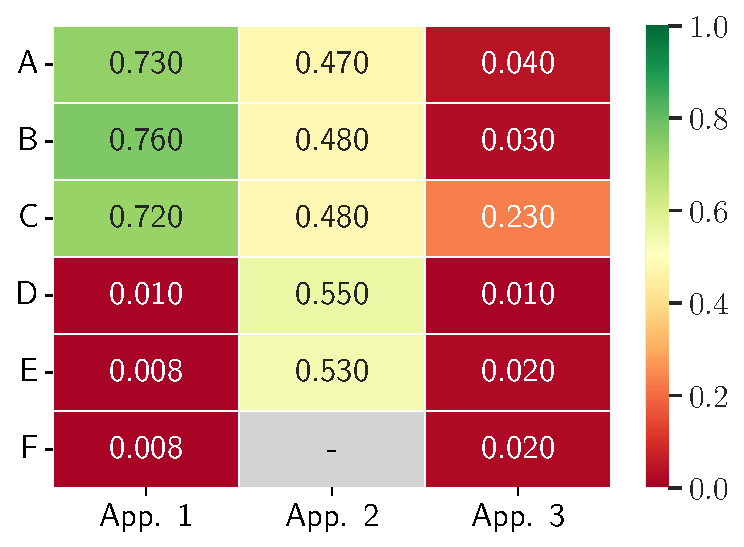
\includegraphics[width=0.75\linewidth]{figures/02_performance_portability/example_diss_eff_heat.pdf}
    \caption{%
    An example visualization of the architectural efficiencies (higher is better) of \autoref{tab:example_effs} as a heatmap. 
    This visualization makes it easy to spot the overall behavior of the three example applications. 
    }
    \label{fig:vis_example_effs}
\end{figure}

Such heatmaps make it easy to see the different application characteristics at a glance, including the cases where an application does not support a hardware platform. 
However, care must be taken to scale the heatmap to the same range, in case of performance efficiencies, the range $\interval{0}{1}$, regardless of the actual values, to make different heatmaps easier comparable. 

However, visualizing the performance portability metrics without losing or obscuring too much information is more difficult. 
In their paper, \citet{sewall_interpreting_2020} compared different visualization techniques for their \pp metric and discussed their advantages and disadvantages. 
They concluded that established visualization techniques like box plots, histograms, probability density functions, or violin plots in theory work, but they all lose or obscure some information, mostly when an application does not support a hardware platform.
They concluded that now-established visualization techniques cannot convey all important information, especially if we factor in the importance of the used platform set in the calculation of \pp. 
Therefore, based on the idea in \cite{deakin_performance_2019}, \citet{sewall_interpreting_2020} proposed the efficiency cascade plots and platform charts. 
Such an example plot for the performance efficiencies in \autoref{tab:example_effs} and performance portability scores of \pp in \autoref{tab:example_perfs} is shown in \autoref{fig:vis_example_pp}.

\begin{figure}
    \centering
    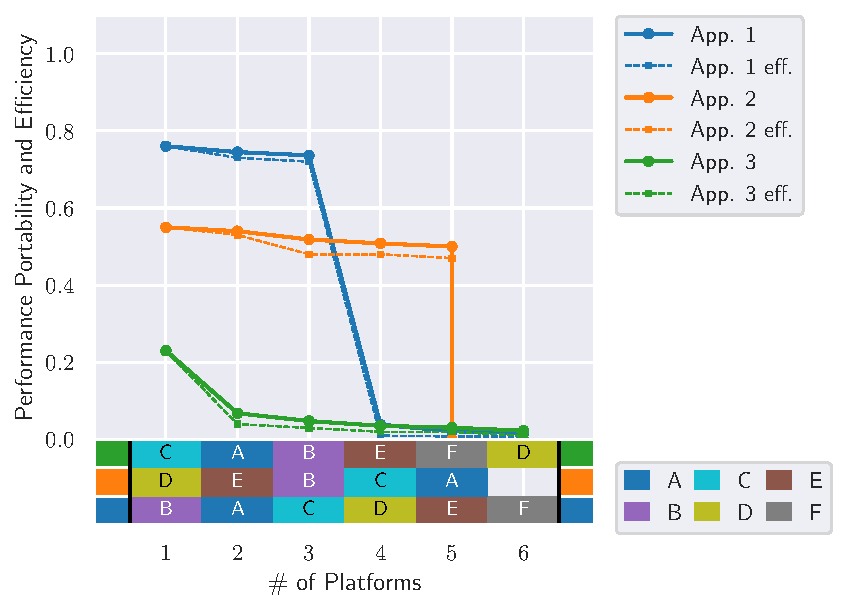
\includegraphics[width=\linewidth]{figures/02_performance_portability/example_diss_eff_cascade.pdf}
    \caption{%
    An example visualization of the architectural efficiencies of \autoref{tab:example_effs} and performance portability scores of \autoref{tab:example_pp} for \pp for the three example applications as proposed by \citet{sewall_interpreting_2020}. 
    This plot can help us to determine the set of platforms best supported by some applications. 
    }
    \label{fig:vis_example_pp}
\end{figure}

Creating an efficiency cascade plot works as follows. 
First, each application's \pp and efficiency values are gathered using all hardware platforms. 
Afterward, the platform with the smallest remaining efficiency is removed and the now-reduced platform set as a new baseline to calculate the next \pp score. 
This process is repeated until only one platform, the best-performing platform for the current application, is left in the platform set. 
These values are then plotted from right to left, resulting in a monotonically decreasing plot of the performance portability scores and efficiencies. 
Alternatively, the new \enquote{P3 explorer} project can be used to automate the creation of a efficiency cascade plot~\cite{smith_p3_2024, smith_p3-explorerp3-explorergithubio_2024}. 

As discussed by \citet{sewall_interpreting_2020, pennycook_navigating_2021}, this plot can be used to draw many different conclusions from the raw \pp and performance efficiency values. 
Applications for which the efficiency cascade plot extends further to the right support more hardware platforms and are, therefore, more portable. 
Also, we can directly see how many platforms are supported and which platforms have the highest performance efficiencies. 
This can help us identify whether our application's performance in one architectural class is lackluster and needs to be addressed. 
One drawback of the efficiency cascade plots is that one must be careful since the order of hardware platforms in the platform charts at the bottom of the plot may differ for each application. 

For an example, we can look at \autoref{fig:vis_example_pp}. 
For application one, we see that the platforms from the first architectural class are supported best, followed by a sharp decline in performance portability after adding platforms from the second class. 
On the other hand, application two's performance portability scores are, on average, better for more hardware platforms until platform F is added, which results in a score of zero, shown by a vertical decline in the plot. 
Application three also shows bad performance portability scores for all hardware platforms, as already discussed. 


The efficiency cascade plots were created only with \pp in mind. 
Creating the same plot for the \mpp metric is not directly possible since, per \autoref{def:mpp}, only platforms with the same architectural class should be used to calculate \mpp. 
However, if we relax this restriction and use all platforms when calculating \mpp, we can also create an efficiency cascade plot for scores retrieved via \mpp. 

\begin{figure}
    \centering
    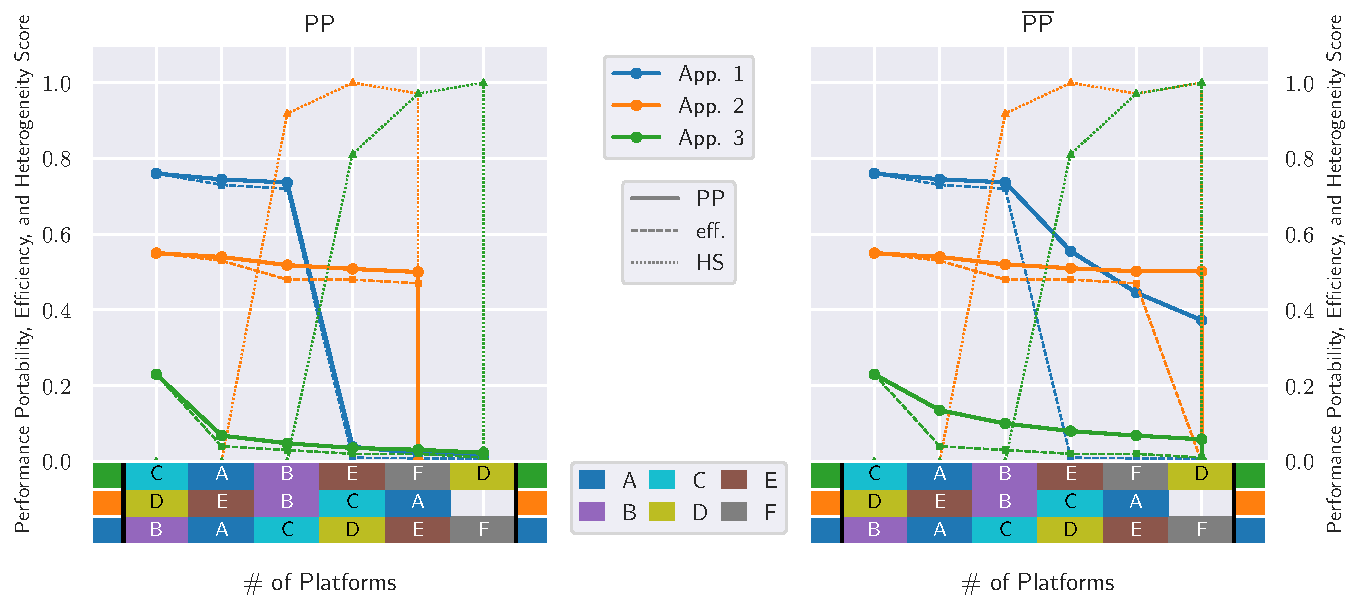
\includegraphics[width=\linewidth]{figures/02_performance_portability/example_diss_eff_cascade_both_HS.pdf}
    \caption{%
    An example visualization of the architectural efficiencies of \autoref{tab:example_effs} and performance portability scores of \autoref{tab:example_pp} for the three example applications as proposed by \citet{sewall_interpreting_2020}. 
    On the left-hand side, the scores for \pp proposed by \citet{pennycook_implications_2019} are plotted, and on the right-hand side, the scores for \mpp proposed by \citet{marowka_comparison_2023}. 
    Additionally, both plots contain the newly proposed heterogeneity score $HS$ (\autoref{def:hetero_score}) as dotted lines. 
    }
    \label{fig:vis_example_both_hs}
\end{figure}

\autoref{fig:vis_example_both_hs} displays the same plot as \autoref{fig:vis_example_pp} but now showing both performance portability metrics, \pp (left-hand side) and \mpp (right-hand side). 
Additionally, the newly proposed heterogeneity score $HS$ is added as dotted lines. 
The plot on the left shows that while application one has a high \pp score, its heterogeneity score is zero in our example, meaning only a single architectural class is highly optimized. 
On the other hand, application two's \pp score is lower, but its heterogeneity score is higher, meaning its \pp score of roughly $\num{0.5}$ is not caused by only one architectural class being optimized but multiple. 
This new heterogeneity score plot nicely complements the efficiency cascade plot and the platform chart, making the results easier and better interpretable. 

Looking at the efficiency cascade plot of the \mpp metric, we can see that due to the usage of the arithmetic mean, the correlation between the \mpp values and the corresponding performance efficiencies is not as high as with the \pp metric. 

